\documentclass{beamer}

\usepackage[latin1]{inputenc}
\usepackage{algorithmic}
\usepackage{amsmath}
\usepackage{graphicx}

\title{Bayesian Particle Filter Tracking with CUDA}
\author{Geoffrey Ulman}
\date{May 6, 2010}
\begin{document}

%%%%%%%%%%%%%%%%%%%%%%%%%%%%%%%%%%%%%%%%%%%%%%%%%%%%

\begin{frame}
\titlepage
\end{frame}

%%%%%%%%%%%%%%%%%%%%%%%%%%%%%%%%%%%%%%%%%%%%%%%%%%%%

\begin{frame}{Motivating Example}

A submarine with a hydrophone (passive sonar) is following another
ship using the direction of the sound from the ship's engine.

\vspace{1cm}

How can the series of bearing observations from the hydrophone be
used to estimate the second ship's position and velocity?

\end{frame}

%%%%%%%%%%%%%%%%%%%%%%%%%%%%%%%%%%%%%%%%%%%%%%%%%%%%

\begin{frame}{Likelihood Function}
\begin{equation}
L(y|x) = P( Y=y | X=x ) \hspace{0.5cm} \mbox{for} \hspace{0.5cm} x \in S
\end{equation}

\vspace{1cm}

\begin{itemize}
\item \(X\) Random variable on \(S\)
\item \(Y\) Random variable on measurment space \(H\)
\item \(P(\cdot|x)\) Probability density function on \(H\)
\item \(P(y|\cdot)\) Likelihood function relating \(X\) and \(Y\)
\end{itemize}

\end{frame}

%%%%%%%%%%%%%%%%%%%%%%%%%%%%%%%%%%%%%%%%%%%%%%%%%%%%

\begin{frame}{Bayesian Inference}

\begin{equation}
P(x|y) = \frac{L(y|x)P(x)}{P(y)} = \frac{L(y|x)P(x)}{\int \! L(y|x)P(x) \, dx}
\end{equation}

\vspace{1cm}

\begin{itemize}
\item Observation \(y\) is fixed, \(x\) represents possible target states
\item \(P(x)\) Prior probability density function on true target state
\item \(P(x|y)\) Posterior distribution given observation \(y\)
\end{itemize}

\end{frame}

%%%%%%%%%%%%%%%%%%%%%%%%%%%%%%%%%%%%%%%%%%%%%%%%%%%%


\begin{frame}{Prior Distribution}

\begin{figure}
\centering
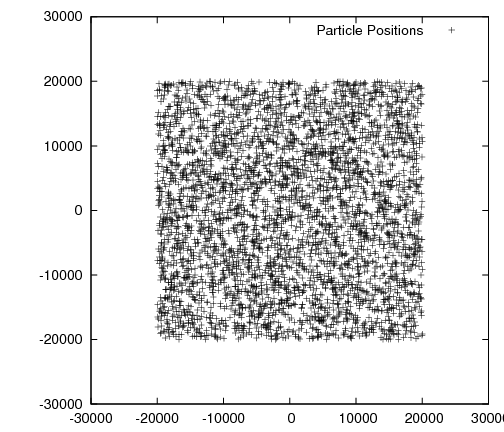
\includegraphics[width=0.7\textwidth]{data/particles_prior.png}
\caption{Prior Particle Position Distribution}
\end{figure}

\end{frame}


%%%%%%%%%%%%%%%%%%%%%%%%%%%%%%%%%%%%%%%%%%%%%%%%%%%%


\begin{frame}{Information Update}

\begin{figure}
\centering
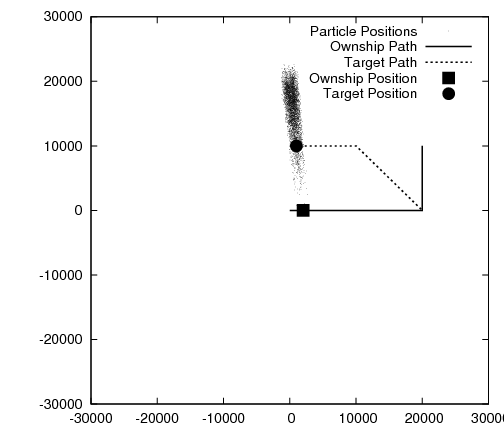
\includegraphics[width=0.7\textwidth]{data/particles_azimuth_obs.png}
\caption{Posterior Particle Position Distribution after Azimuth Observation}
\end{figure}

\end{frame}


%%%%%%%%%%%%%%%%%%%%%%%%%%%%%%%%%%%%%%%%%%%%%%%%%%%%


\begin{frame}{Motion Model}

\begin{figure}
\centering
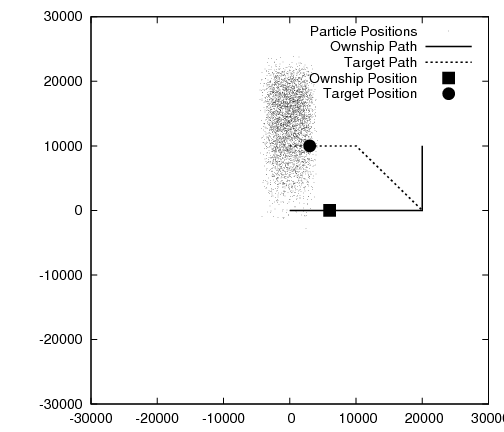
\includegraphics[width=0.7\textwidth]{data/particles_motion.png}
\caption{Posterior Particle Position Distribution after Motion Update}
\end{figure}

\end{frame}


%%%%%%%%%%%%%%%%%%%%%%%%%%%%%%%%%%%%%%%%%%%%%%%%%%%%


\begin{frame}{Resampling}

\begin{equation}\label{resample1}
C = \frac{n}{\sum_{i=0}^{n} w_{i}}
\end{equation}

\begin{equation}\label{resample2}
w_{i}=C w_{j}
\end{equation}

\begin{equation}\label{resample3}
w_{i}=\verb!floor!(C\sum_{j=0}^{i} w_{j})
\end{equation}

\end{frame}


%%%%%%%%%%%%%%%%%%%%%%%%%%%%%%%%%%%%%%%%%%%%%%%%%%%%

\end{document}
